% Options for packages loaded elsewhere
\PassOptionsToPackage{unicode}{hyperref}
\PassOptionsToPackage{hyphens}{url}
\documentclass[
]{book}
\usepackage{xcolor}
\usepackage{amsmath,amssymb}
\setcounter{secnumdepth}{5}
\usepackage{iftex}
\ifPDFTeX
  \usepackage[T1]{fontenc}
  \usepackage[utf8]{inputenc}
  \usepackage{textcomp} % provide euro and other symbols
\else % if luatex or xetex
  \usepackage{unicode-math} % this also loads fontspec
  \defaultfontfeatures{Scale=MatchLowercase}
  \defaultfontfeatures[\rmfamily]{Ligatures=TeX,Scale=1}
\fi
\usepackage{lmodern}
\ifPDFTeX\else
  % xetex/luatex font selection
\fi
% Use upquote if available, for straight quotes in verbatim environments
\IfFileExists{upquote.sty}{\usepackage{upquote}}{}
\IfFileExists{microtype.sty}{% use microtype if available
  \usepackage[]{microtype}
  \UseMicrotypeSet[protrusion]{basicmath} % disable protrusion for tt fonts
}{}
\makeatletter
\@ifundefined{KOMAClassName}{% if non-KOMA class
  \IfFileExists{parskip.sty}{%
    \usepackage{parskip}
  }{% else
    \setlength{\parindent}{0pt}
    \setlength{\parskip}{6pt plus 2pt minus 1pt}}
}{% if KOMA class
  \KOMAoptions{parskip=half}}
\makeatother
\usepackage{color}
\usepackage{fancyvrb}
\newcommand{\VerbBar}{|}
\newcommand{\VERB}{\Verb[commandchars=\\\{\}]}
\DefineVerbatimEnvironment{Highlighting}{Verbatim}{commandchars=\\\{\}}
% Add ',fontsize=\small' for more characters per line
\usepackage{framed}
\definecolor{shadecolor}{RGB}{248,248,248}
\newenvironment{Shaded}{\begin{snugshade}}{\end{snugshade}}
\newcommand{\AlertTok}[1]{\textcolor[rgb]{0.94,0.16,0.16}{#1}}
\newcommand{\AnnotationTok}[1]{\textcolor[rgb]{0.56,0.35,0.01}{\textbf{\textit{#1}}}}
\newcommand{\AttributeTok}[1]{\textcolor[rgb]{0.13,0.29,0.53}{#1}}
\newcommand{\BaseNTok}[1]{\textcolor[rgb]{0.00,0.00,0.81}{#1}}
\newcommand{\BuiltInTok}[1]{#1}
\newcommand{\CharTok}[1]{\textcolor[rgb]{0.31,0.60,0.02}{#1}}
\newcommand{\CommentTok}[1]{\textcolor[rgb]{0.56,0.35,0.01}{\textit{#1}}}
\newcommand{\CommentVarTok}[1]{\textcolor[rgb]{0.56,0.35,0.01}{\textbf{\textit{#1}}}}
\newcommand{\ConstantTok}[1]{\textcolor[rgb]{0.56,0.35,0.01}{#1}}
\newcommand{\ControlFlowTok}[1]{\textcolor[rgb]{0.13,0.29,0.53}{\textbf{#1}}}
\newcommand{\DataTypeTok}[1]{\textcolor[rgb]{0.13,0.29,0.53}{#1}}
\newcommand{\DecValTok}[1]{\textcolor[rgb]{0.00,0.00,0.81}{#1}}
\newcommand{\DocumentationTok}[1]{\textcolor[rgb]{0.56,0.35,0.01}{\textbf{\textit{#1}}}}
\newcommand{\ErrorTok}[1]{\textcolor[rgb]{0.64,0.00,0.00}{\textbf{#1}}}
\newcommand{\ExtensionTok}[1]{#1}
\newcommand{\FloatTok}[1]{\textcolor[rgb]{0.00,0.00,0.81}{#1}}
\newcommand{\FunctionTok}[1]{\textcolor[rgb]{0.13,0.29,0.53}{\textbf{#1}}}
\newcommand{\ImportTok}[1]{#1}
\newcommand{\InformationTok}[1]{\textcolor[rgb]{0.56,0.35,0.01}{\textbf{\textit{#1}}}}
\newcommand{\KeywordTok}[1]{\textcolor[rgb]{0.13,0.29,0.53}{\textbf{#1}}}
\newcommand{\NormalTok}[1]{#1}
\newcommand{\OperatorTok}[1]{\textcolor[rgb]{0.81,0.36,0.00}{\textbf{#1}}}
\newcommand{\OtherTok}[1]{\textcolor[rgb]{0.56,0.35,0.01}{#1}}
\newcommand{\PreprocessorTok}[1]{\textcolor[rgb]{0.56,0.35,0.01}{\textit{#1}}}
\newcommand{\RegionMarkerTok}[1]{#1}
\newcommand{\SpecialCharTok}[1]{\textcolor[rgb]{0.81,0.36,0.00}{\textbf{#1}}}
\newcommand{\SpecialStringTok}[1]{\textcolor[rgb]{0.31,0.60,0.02}{#1}}
\newcommand{\StringTok}[1]{\textcolor[rgb]{0.31,0.60,0.02}{#1}}
\newcommand{\VariableTok}[1]{\textcolor[rgb]{0.00,0.00,0.00}{#1}}
\newcommand{\VerbatimStringTok}[1]{\textcolor[rgb]{0.31,0.60,0.02}{#1}}
\newcommand{\WarningTok}[1]{\textcolor[rgb]{0.56,0.35,0.01}{\textbf{\textit{#1}}}}
\usepackage{longtable,booktabs,array}
\usepackage{calc} % for calculating minipage widths
% Correct order of tables after \paragraph or \subparagraph
\usepackage{etoolbox}
\makeatletter
\patchcmd\longtable{\par}{\if@noskipsec\mbox{}\fi\par}{}{}
\makeatother
% Allow footnotes in longtable head/foot
\IfFileExists{footnotehyper.sty}{\usepackage{footnotehyper}}{\usepackage{footnote}}
\makesavenoteenv{longtable}
\usepackage{graphicx}
\makeatletter
\newsavebox\pandoc@box
\newcommand*\pandocbounded[1]{% scales image to fit in text height/width
  \sbox\pandoc@box{#1}%
  \Gscale@div\@tempa{\textheight}{\dimexpr\ht\pandoc@box+\dp\pandoc@box\relax}%
  \Gscale@div\@tempb{\linewidth}{\wd\pandoc@box}%
  \ifdim\@tempb\p@<\@tempa\p@\let\@tempa\@tempb\fi% select the smaller of both
  \ifdim\@tempa\p@<\p@\scalebox{\@tempa}{\usebox\pandoc@box}%
  \else\usebox{\pandoc@box}%
  \fi%
}
% Set default figure placement to htbp
\def\fps@figure{htbp}
\makeatother
\setlength{\emergencystretch}{3em} % prevent overfull lines
\providecommand{\tightlist}{%
  \setlength{\itemsep}{0pt}\setlength{\parskip}{0pt}}
\usepackage[]{natbib}
\bibliographystyle{plainnat}
\usepackage{booktabs}
\usepackage{bookmark}
\IfFileExists{xurl.sty}{\usepackage{xurl}}{} % add URL line breaks if available
\urlstyle{same}
\hypersetup{
  pdftitle={Tecnologia e Inovação},
  pdfauthor={Juliana Costa-Silva},
  hidelinks,
  pdfcreator={LaTeX via pandoc}}

\title{Tecnologia e Inovação}
\author{Juliana Costa-Silva}
\date{2026-03-12}

\usepackage{amsthm}
\newtheorem{theorem}{Theorem}[chapter]
\newtheorem{lemma}{Lemma}[chapter]
\newtheorem{corollary}{Corollary}[chapter]
\newtheorem{proposition}{Proposition}[chapter]
\newtheorem{conjecture}{Conjecture}[chapter]
\theoremstyle{definition}
\newtheorem{definition}{Definition}[chapter]
\theoremstyle{definition}
\newtheorem{example}{Example}[chapter]
\theoremstyle{definition}
\newtheorem{exercise}{Exercise}[chapter]
\theoremstyle{definition}
\newtheorem{hypothesis}{Hypothesis}[chapter]
\theoremstyle{remark}
\newtheorem*{remark}{Remark}
\newtheorem*{solution}{Solution}
\begin{document}
\maketitle

{
\setcounter{tocdepth}{1}
\tableofcontents
}
\chapter{About}\label{about}

This is a \emph{sample} book written in \textbf{Markdown}. You can use anything that Pandoc's Markdown supports; for example, a math equation \(a^2 + b^2 = c^2\).

\section{Usage}\label{usage}

Each \textbf{bookdown} chapter is an .Rmd file, and each .Rmd file can contain one (and only one) chapter. A chapter \emph{must} start with a first-level heading: \texttt{\#\ A\ good\ chapter}, and can contain one (and only one) first-level heading.

Use second-level and higher headings within chapters like: \texttt{\#\#\ A\ short\ section} or \texttt{\#\#\#\ An\ even\ shorter\ section}.

The \texttt{index.Rmd} file is required, and is also your first book chapter. It will be the homepage when you render the book.

\section{Render book}\label{render-book}

You can render the HTML version of this example book without changing anything:

\begin{enumerate}
\def\labelenumi{\arabic{enumi}.}
\item
  Find the \textbf{Build} pane in the RStudio IDE, and
\item
  Click on \textbf{Build Book}, then select your output format, or select ``All formats'' if you'd like to use multiple formats from the same book source files.
\end{enumerate}

Or build the book from the R console:

\begin{Shaded}
\begin{Highlighting}[]
\NormalTok{bookdown}\SpecialCharTok{::}\FunctionTok{render\_book}\NormalTok{()}
\end{Highlighting}
\end{Shaded}

To render this example to PDF as a \texttt{bookdown::pdf\_book}, you'll need to install XeLaTeX. You are recommended to install TinyTeX (which includes XeLaTeX): \url{https://yihui.org/tinytex/}.

\section{Preview book}\label{preview-book}

As you work, you may start a local server to live preview this HTML book. This preview will update as you edit the book when you save individual .Rmd files. You can start the server in a work session by using the RStudio add-in ``Preview book'', or from the R console:

\begin{Shaded}
\begin{Highlighting}[]
\NormalTok{bookdown}\SpecialCharTok{::}\FunctionTok{serve\_book}\NormalTok{()}
\end{Highlighting}
\end{Shaded}

\chapter{Hello bookdown}\label{hello-bookdown}

All chapters start with a first-level heading followed by your chapter title, like the line above. There should be only one first-level heading (\texttt{\#}) per .Rmd file.

\section{A section}\label{a-section}

All chapter sections start with a second-level (\texttt{\#\#}) or higher heading followed by your section title, like the sections above and below here. You can have as many as you want within a chapter.

\subsection*{An unnumbered section}\label{an-unnumbered-section}
\addcontentsline{toc}{subsection}{An unnumbered section}

Chapters and sections are numbered by default. To un-number a heading, add a \texttt{\{.unnumbered\}} or the shorter \texttt{\{-\}} at the end of the heading, like in this section.

\chapter{Cross-references}\label{cross}

Cross-references make it easier for your readers to find and link to elements in your book.

\section{Chapters and sub-chapters}\label{chapters-and-sub-chapters}

There are two steps to cross-reference any heading:

\begin{enumerate}
\def\labelenumi{\arabic{enumi}.}
\tightlist
\item
  Label the heading: \texttt{\#\ Hello\ world\ \{\#nice-label\}}.

  \begin{itemize}
  \tightlist
  \item
    Leave the label off if you like the automated heading generated based on your heading title: for example, \texttt{\#\ Hello\ world} = \texttt{\#\ Hello\ world\ \{\#hello-world\}}.
  \item
    To label an un-numbered heading, use: \texttt{\#\ Hello\ world\ \{-\#nice-label\}} or \texttt{\{\#\ Hello\ world\ .unnumbered\}}.
  \end{itemize}
\item
  Next, reference the labeled heading anywhere in the text using \texttt{\textbackslash{}@ref(nice-label)}; for example, please see Chapter \ref{cross}.

  \begin{itemize}
  \tightlist
  \item
    If you prefer text as the link instead of a numbered reference use: \hyperref[cross]{any text you want can go here}.
  \end{itemize}
\end{enumerate}

\section{Captioned figures and tables}\label{captioned-figures-and-tables}

Figures and tables \emph{with captions} can also be cross-referenced from elsewhere in your book using \texttt{\textbackslash{}@ref(fig:chunk-label)} and \texttt{\textbackslash{}@ref(tab:chunk-label)}, respectively.

See Figure \ref{fig:nice-fig}.

\begin{Shaded}
\begin{Highlighting}[]
\FunctionTok{par}\NormalTok{(}\AttributeTok{mar =} \FunctionTok{c}\NormalTok{(}\DecValTok{4}\NormalTok{, }\DecValTok{4}\NormalTok{, .}\DecValTok{1}\NormalTok{, .}\DecValTok{1}\NormalTok{))}
\FunctionTok{plot}\NormalTok{(pressure, }\AttributeTok{type =} \StringTok{\textquotesingle{}b\textquotesingle{}}\NormalTok{, }\AttributeTok{pch =} \DecValTok{19}\NormalTok{)}
\end{Highlighting}
\end{Shaded}

\begin{figure}

{\centering 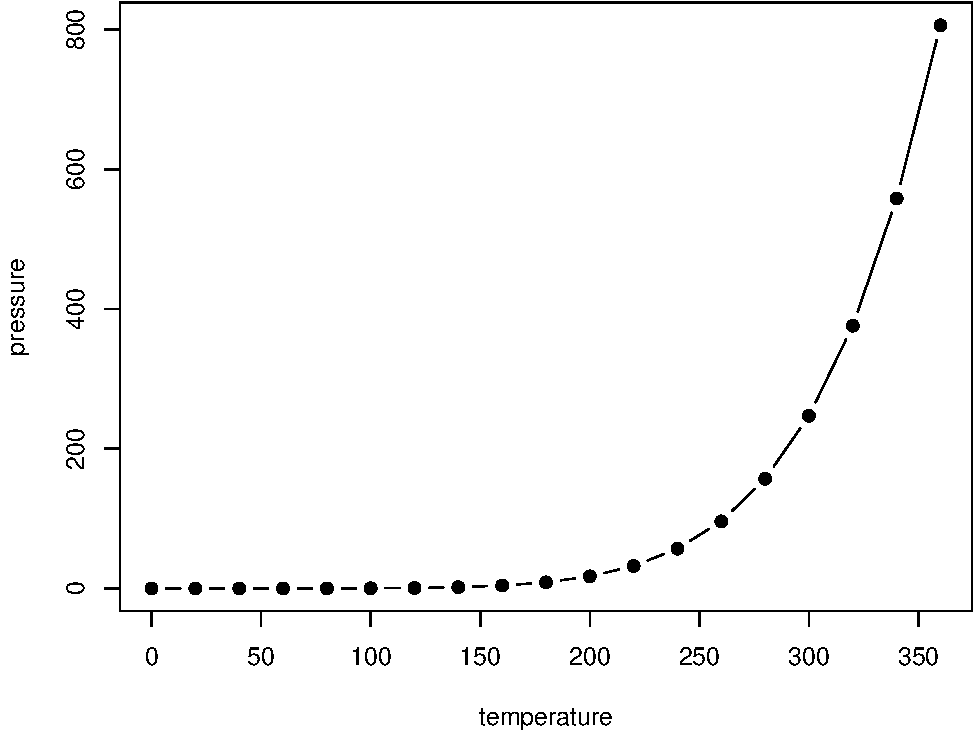
\includegraphics[width=0.8\linewidth,alt={Plot with connected points showing that vapor pressure of mercury increases exponentially as temperature increases.}]{_main_files/figure-latex/nice-fig-1} 

}

\caption{Here is a nice figure!}\label{fig:nice-fig}
\end{figure}

Don't miss Table \ref{tab:nice-tab}.

\begin{Shaded}
\begin{Highlighting}[]
\NormalTok{knitr}\SpecialCharTok{::}\FunctionTok{kable}\NormalTok{(}
  \FunctionTok{head}\NormalTok{(pressure, }\DecValTok{10}\NormalTok{), }\AttributeTok{caption =} \StringTok{\textquotesingle{}Here is a nice table!\textquotesingle{}}\NormalTok{,}
  \AttributeTok{booktabs =} \ConstantTok{TRUE}
\NormalTok{)}
\end{Highlighting}
\end{Shaded}

\begin{table}

\caption{\label{tab:nice-tab}Here is a nice table!}
\centering
\begin{tabular}[t]{rr}
\toprule
temperature & pressure\\
\midrule
0 & 0.0002\\
20 & 0.0012\\
40 & 0.0060\\
60 & 0.0300\\
80 & 0.0900\\
\addlinespace
100 & 0.2700\\
120 & 0.7500\\
140 & 1.8500\\
160 & 4.2000\\
180 & 8.8000\\
\bottomrule
\end{tabular}
\end{table}

\chapter{Aula 2 --- Revolução tecnológica e impactos no trabalho}\label{aula-2-revoluuxe7uxe3o-tecnoluxf3gica-e-impactos-no-trabalho}

\section{Objetivo da aula}\label{objetivo-da-aula}

Compreender como a revolução tecnológica vem transformando o trabalho, os perfis profissionais e as competências exigidas nas organizações, relacionando esse cenário ao campo de atuação do secretariado executivo.

\section{Objetivos específicos}\label{objetivos-especuxedficos}

\begin{itemize}
\tightlist
\item
  entender a transformação tecnológica como processo histórico e organizacional
\item
  analisar como automação, digitalização, inteligência artificial e novas plataformas alteram atividades e ocupações
\item
  discutir os impactos da tecnologia sobre produtividade, emprego, desigualdade e exigências de qualificação
\item
  identificar riscos e oportunidades para profissionais do secretariado executivo
\item
  refletir sobre competências humanas e digitais que tendem a ganhar valor nos próximos anos
\end{itemize}

\begin{center}\rule{0.5\linewidth}{0.5pt}\end{center}

\chapter{1. Visão geral da aula}\label{visuxe3o-geral-da-aula}

A proposta desta aula é construir um caminho lógico que parte de uma ideia simples: \textbf{a tecnologia não afeta apenas máquinas e sistemas; ela reorganiza o trabalho, redefine funções e muda o valor de certas competências}.

Para isso, a aula combina três perspectivas complementares:

\begin{enumerate}
\def\labelenumi{\arabic{enumi}.}
\tightlist
\item
  \textbf{A perspectiva organizacional}, baseada no texto \emph{O impacto das tecnologias digitais nos processos de gestão de pessoas}, que mostra como as tecnologias digitais transformam processos internos, descentralizam operações, aumentam a autonomia e também geram tensões, resistência e necessidade de novas competências.
\item
  \textbf{A perspectiva econômica de longo prazo}, baseada no relatório do FMI \emph{Technology and the Future of Work}, que mostra que a tecnologia historicamente elevou produtividade e renda, mas também provocou deslocamentos ocupacionais, polarização salarial e queda relativa da participação do trabalho em alguns contextos.
\item
  \textbf{A perspectiva prospectiva do mercado de trabalho}, baseada no \emph{Future of Jobs Report 2025} do Fórum Econômico Mundial, que aponta tendências concretas até 2030, incluindo crescimento de ocupações tecnológicas e verdes, declínio de funções administrativas rotineiras e valorização de competências analíticas, tecnológicas e socioemocionais.
\end{enumerate}

O ponto central da aula é o seguinte:

\begin{quote}
a tecnologia não elimina apenas empregos; ela transforma tarefas, reconfigura profissões e exige reposicionamento profissional.
\end{quote}

Esse ponto é especialmente importante para o secretariado executivo, porque se trata de uma área tradicionalmente associada à gestão da informação, comunicação, organização de rotinas, apoio à liderança e articulação entre pessoas, setores e processos. Justamente por isso, é uma área fortemente impactada por automação e IA, mas também uma área com grande potencial de reinvenção.

\begin{center}\rule{0.5\linewidth}{0.5pt}\end{center}

\chapter{2. Organização da aula em blocos}\label{organizauxe7uxe3o-da-aula-em-blocos}

\section{Bloco 1 --- Abertura e problematização}\label{bloco-1-abertura-e-problematizauxe7uxe3o}

\textbf{Tempo sugerido:} 10 minutos

\subsection{Pergunta disparadora}\label{pergunta-disparadora}

Pergunte à turma:

\textbf{Quais atividades de trabalho hoje já foram parcial ou totalmente substituídas por sistemas digitais, aplicativos, automação ou inteligência artificial}

Anote exemplos trazidos pelos estudantes, como:
- atendimento automatizado
- agendamento online
- emissão automática de documentos
- sistemas de gestão empresarial
- chatbots
- videoconferência
- tradução automática
- ferramentas de IA para redação, resumo e organização de informação

\subsection{Objetivo deste momento}\label{objetivo-deste-momento}

Mostrar que a revolução tecnológica não é um evento distante. Ela já está presente em tarefas administrativas, comunicação corporativa, gestão documental, suporte a decisões e relacionamento com clientes e equipes.

\subsection{Gancho para a aula}\label{gancho-para-a-aula}

Explique que, no passado, a preocupação maior era a mecanização do trabalho físico. Hoje, além disso, existe a automação de tarefas cognitivas e rotineiras. Isso afeta diretamente ocupações ligadas à informação, ao apoio administrativo e à coordenação organizacional.

\begin{center}\rule{0.5\linewidth}{0.5pt}\end{center}

\section{Bloco 2 --- Da informatização à transformação do trabalho}\label{bloco-2-da-informatizauxe7uxe3o-uxe0-transformauxe7uxe3o-do-trabalho}

\textbf{Tempo sugerido:} 15 minutos

\subsection{Ideia central}\label{ideia-central}

A tecnologia, no contexto organizacional, não deve ser entendida apenas como conjunto de equipamentos. Ela altera a forma de trabalhar, tomar decisões, comunicar, controlar processos e distribuir responsabilidades.

\subsection{Desenvolvimento conceitual}\label{desenvolvimento-conceitual}

Com base no artigo sobre tecnologias digitais e gestão de pessoas, apresente a seguinte evolução:

\subsection{2.1. Da burocracia manual à operação digital}\label{da-burocracia-manual-uxe0-operauxe7uxe3o-digital}

Antes, várias atividades organizacionais dependiam de papel, arquivos físicos, comunicação lenta e forte centralização.

Com a digitalização:
- a informação circula com mais rapidez
- processos ficam registrados em sistemas
- gestores e funcionários acessam dados diretamente
- atividades antes concentradas em um setor passam a ser distribuídas

\subsection{2.2. O RH como exemplo de transformação}\label{o-rh-como-exemplo-de-transformauxe7uxe3o}

O artigo-base mostra bem isso ao discutir a área de gestão de pessoas.

A tecnologia:
- agiliza recrutamento e seleção
- automatiza rotinas administrativas
- melhora registro e acompanhamento de desempenho
- facilita comunicação entre setores
- amplia acesso à informação
- descentraliza operações

Mas também cria desafios:
- resistência à mudança
- pressão por adaptação rápida
- necessidade de qualificação
- novas formas de vigilância e controle
- risco de desumanização de processos

\subsection{Comparação importante para a turma}\label{comparauxe7uxe3o-importante-para-a-turma}

Faça uma comparação simples:

\begin{itemize}
\tightlist
\item
  \textbf{modelo antigo:} a informação fica guardada em setores e depende de mediação humana constante
\item
  \textbf{modelo digital:} a informação circula mais livremente, mas exige interpretação, julgamento, curadoria e responsabilidade
\end{itemize}

\subsection{Conexão com o secretariado executivo}\label{conexuxe3o-com-o-secretariado-executivo}

Nesse ponto, destaque que o secretariado executivo historicamente ocupa uma posição estratégica justamente porque lida com:
- organização da informação
- comunicação institucional
- apoio à gestão
- articulação entre pessoas e setores
- acompanhamento de processos

Ou seja, a profissão não está fora da transformação digital; ela está no centro dela.

\begin{center}\rule{0.5\linewidth}{0.5pt}\end{center}

\section{Bloco 3 --- O que a história econômica mostra sobre tecnologia e trabalho}\label{bloco-3-o-que-a-histuxf3ria-econuxf4mica-mostra-sobre-tecnologia-e-trabalho}

\textbf{Tempo sugerido:} 20 minutos

\subsection{Ideia central}\label{ideia-central-1}

O relatório do FMI ajuda a desfazer uma visão simplista de que ``tecnologia sempre destrói empregos''. A questão é mais complexa.

\subsection{3.1. Tecnologia como motor de crescimento}\label{tecnologia-como-motor-de-crescimento}

Historicamente, a tecnologia elevou a produtividade e sustentou aumentos no padrão de vida. Inovações como máquina a vapor, eletricidade, automóvel, computador e internet estiveram associadas a crescimento econômico e aumento da renda média.

\subsection{3.2. Mais produtividade não significa automaticamente menos trabalho}\label{mais-produtividade-nuxe3o-significa-automaticamente-menos-trabalho}

O relatório mostra que, no longo prazo, o avanço tecnológico esteve associado a:
- maior produtividade
- crescimento do emprego agregado
- aumento dos salários reais em vários contextos

Isso acontece porque novas tecnologias eliminam algumas tarefas, mas criam outras, além de gerar novos setores, produtos e serviços.

\subsection{3.3. O problema está na transição}\label{o-problema-estuxe1-na-transiuxe7uxe3o}

Mesmo quando a economia cresce, a transição pode ser dolorosa. Algumas pessoas e grupos são mais afetados do que outros.

Explique aos estudantes:

A tecnologia tende a produzir três movimentos ao mesmo tempo:
1. cria novas oportunidades
2. reduz ou transforma ocupações existentes
3. exige novas habilidades para acompanhar a mudança

\subsection{3.4. Polarização do trabalho}\label{polarizauxe7uxe3o-do-trabalho}

O FMI chama atenção para um fenômeno importante: a \textbf{polarização}.

Em termos simples:
- ocupações muito rotineiras ficam mais expostas à automação
- ocupações de alta qualificação tendem a capturar mais ganhos
- ocupações intermediárias podem perder espaço

Isso ajuda a entender por que funções administrativas repetitivas, baseadas em registro, conferência e processamento padronizado de informação, se tornam mais vulneráveis.

\subsection{3.5. Queda relativa da participação do trabalho}\label{queda-relativa-da-participauxe7uxe3o-do-trabalho}

Outro ponto relevante do relatório é que a tecnologia pode aumentar a participação do capital na renda quando máquinas, sistemas e infraestrutura tecnológica substituem parte do trabalho humano.

Não significa que o trabalho deixa de existir.
Significa que o valor econômico pode se deslocar para quem controla tecnologia, dados, plataformas e ativos.

\subsection{Comparação didática}\label{comparauxe7uxe3o-diduxe1tica}

Você pode dizer em aula:

\begin{quote}
no século XX, a automação afetava mais o esforço físico repetitivo. No século XXI, ela também afeta o trabalho informacional repetitivo.
\end{quote}

Isso aproxima diretamente o debate do universo administrativo e secretarial.

\begin{center}\rule{0.5\linewidth}{0.5pt}\end{center}

\section{Bloco 4 --- O que muda entre 2025 e 2030}\label{bloco-4-o-que-muda-entre-2025-e-2030}

\textbf{Tempo sugerido:} 20 minutos

\subsection{Ideia central}\label{ideia-central-2}

O relatório do Fórum Econômico Mundial mostra tendências concretas para o futuro próximo do trabalho. Aqui a discussão fica mais tangível para os estudantes.

\subsection{4.1. Quais tendências mais transformam as organizações}\label{quais-tenduxeancias-mais-transformam-as-organizauxe7uxf5es}

Segundo o relatório, entre os principais vetores de transformação estão:
- ampliação do acesso digital
- IA e processamento de informação
- robótica e automação
- custo de vida e incerteza econômica
- transição verde
- mudanças demográficas

\subsection{4.2. Crescimento e destruição de empregos acontecem ao mesmo tempo}\label{crescimento-e-destruiuxe7uxe3o-de-empregos-acontecem-ao-mesmo-tempo}

O relatório projeta, até 2030, um cenário de forte transformação estrutural:
- criação de novas ocupações
- deslocamento de ocupações existentes
- crescimento líquido do emprego, mas com intensa reorganização das funções

Esse é um ponto importante para enfatizar:

\begin{quote}
o problema não é apenas quantos empregos existirão, mas quais empregos crescerão, quais perderão espaço e que competências serão exigidas.
\end{quote}

\subsection{4.3. Funções em crescimento}\label{funuxe7uxf5es-em-crescimento}

Entre os grupos ocupacionais que crescem, o relatório destaca:
- especialistas em IA e aprendizado de máquina
- especialistas em big data
- desenvolvedores de software
- especialistas em segurança da informação
- analistas de dados
- engenheiros ambientais e de energia renovável
- profissionais da educação e do cuidado

\subsection{4.4. Funções em declínio}\label{funuxe7uxf5es-em-decluxednio}

Entre as funções com maior tendência de declínio, aparecem justamente várias funções administrativas e clericais, como:
- digitadores
- caixas e bilheteiros
- atendentes bancários
- auxiliares administrativos
- secretários executivos e assistentes administrativos
- profissionais de registro, controle e escrituração padronizada

\subsection{Ponto de atenção pedagógico}\label{ponto-de-atenuxe7uxe3o-pedaguxf3gico}

Aqui é essencial evitar uma leitura alarmista.

O relatório \textbf{não diz que toda atuação administrativa desaparecerá}.
Ele mostra que \textbf{tarefas administrativas rotineiras, previsíveis e padronizáveis estão sob maior risco}.

\subsection{4.5. O que isso significa para o secretariado executivo}\label{o-que-isso-significa-para-o-secretariado-executivo}

Significa que o diferencial profissional deixa de estar no simples apoio operacional e passa a estar em atividades como:
- gestão qualificada da informação
- comunicação estratégica
- mediação entre pessoas e áreas
- organização de fluxos e prioridades
- apoio a decisões
- curadoria de conteúdo e documentos
- coordenação de agendas complexas
- domínio de ferramentas digitais
- atuação com discrição, julgamento e inteligência relacional

\begin{center}\rule{0.5\linewidth}{0.5pt}\end{center}

\section{Bloco 5 --- Competências do futuro e reposicionamento profissional}\label{bloco-5-competuxeancias-do-futuro-e-reposicionamento-profissional}

\textbf{Tempo sugerido:} 15 minutos

\subsection{Ideia central}\label{ideia-central-3}

Se tarefas mudam, o valor profissional também muda.

\subsection{5.1. Competências em alta}\label{competuxeancias-em-alta}

O relatório do WEF mostra crescimento especialmente forte de competências como:
- IA e big data
- redes e cibersegurança
- letramento tecnológico
- pensamento analítico
- pensamento criativo
- resiliência, flexibilidade e agilidade
- curiosidade e aprendizagem contínua
- liderança e influência social
- gestão de talentos
- consciência ambiental

\subsection{5.2. Leitura crítica para o secretariado executivo}\label{leitura-cruxedtica-para-o-secretariado-executivo}

O profissional do secretariado não precisa necessariamente se tornar programador ou cientista de dados.

Mas precisa, cada vez mais:
- compreender ecossistemas digitais
- interagir bem com sistemas inteligentes
- interpretar informações com senso crítico
- produzir comunicação qualificada
- apoiar lideranças em ambientes complexos
- aprender continuamente

\subsection{5.3. O que perde valor relativo}\label{o-que-perde-valor-relativo}

O relatório também mostra redução relativa de valor em habilidades muito associadas a repetição mecânica e execução previsível.

No campo administrativo, isso significa perda de centralidade de atividades como:
- digitação simples
- controle manual repetitivo
- arquivamento convencional
- preenchimento operacional sem análise
- comunicação meramente transmissiva

\subsection{Comparação útil para a turma}\label{comparauxe7uxe3o-uxfatil-para-a-turma}

Use a seguinte comparação:

\begin{itemize}
\tightlist
\item
  \textbf{perfil antigo valorizado:} executar rotinas com precisão
\item
  \textbf{perfil atual e futuro valorizado:} interpretar contextos, organizar fluxos, usar tecnologia, comunicar com qualidade e apoiar decisões
\end{itemize}

\begin{center}\rule{0.5\linewidth}{0.5pt}\end{center}

\chapter{3. Síntese interpretativa para condução da explicação}\label{suxedntese-interpretativa-para-conduuxe7uxe3o-da-explicauxe7uxe3o}

\section{3.1. O que os três textos mostram em conjunto}\label{o-que-os-truxeas-textos-mostram-em-conjunto}

\subsection{O artigo-base}\label{o-artigo-base}

Mostra a transformação da gestão interna das organizações e destaca que a tecnologia:
- democratiza informação
- descentraliza processos
- amplia autonomia
- exige adaptação
- pode tanto humanizar quanto endurecer relações de trabalho, dependendo da forma de implementação

\subsection{O relatório do FMI}\label{o-relatuxf3rio-do-fmi}

Mostra que:
- tecnologia historicamente aumenta produtividade e renda
- não há evidência simples de desaparecimento geral do trabalho
- os ganhos são distribuídos de forma desigual
- a transição pesa mais sobre atividades rotineiras e trabalhadores menos preparados para requalificação

\subsection{O relatório do WEF}\label{o-relatuxf3rio-do-wef}

Mostra que:
- a transformação já está em curso
- funções tecnológicas e verdes crescem rapidamente
- funções clericais e administrativas rotineiras perdem espaço
- as competências mais valorizadas combinam tecnologia, análise e habilidades humanas

\section{3.2. Conclusão conceitual da aula}\label{conclusuxe3o-conceitual-da-aula}

A revolução tecnológica não deve ser interpretada apenas como substituição de pessoas por máquinas.

Ela é, principalmente, uma \textbf{reorganização do valor do trabalho}.

Trabalhos baseados em repetição, previsibilidade e baixo grau de julgamento tendem a ser mais facilmente automatizados.

Trabalhos baseados em:
- interpretação
- comunicação
- tomada de decisão
- articulação entre atores
- confiança
- criatividade
- adaptabilidade

continuam essenciais e podem ganhar ainda mais valor.

Esse é o ponto-chave para o secretariado executivo.

\begin{center}\rule{0.5\linewidth}{0.5pt}\end{center}

\chapter{4. Aplicação direta ao curso de Secretariado Executivo}\label{aplicauxe7uxe3o-direta-ao-curso-de-secretariado-executivo}

\section{4.1. Riscos para a área}\label{riscos-para-a-uxe1rea}

\begin{itemize}
\tightlist
\item
  automação de tarefas de agenda, registro e triagem
\item
  uso crescente de assistentes virtuais e sistemas integrados
\item
  redução da demanda por funções puramente operacionais
\item
  pressão por produtividade e disponibilidade constante
\end{itemize}

\section{4.2. Oportunidades para a área}\label{oportunidades-para-a-uxe1rea}

\begin{itemize}
\tightlist
\item
  gestão inteligente da informação
\item
  organização de fluxos híbridos de trabalho
\item
  apoio executivo em ambiente digital
\item
  mediação comunicacional entre setores e públicos
\item
  curadoria de documentos e relatórios
\item
  uso estratégico de IA para síntese, organização e apoio à comunicação
\item
  coordenação de eventos, agendas e processos complexos
\item
  atuação com governança, confidencialidade e confiabilidade
\end{itemize}

\section{4.3. Reposicionamento desejável do estudante}\label{reposicionamento-desejuxe1vel-do-estudante}

Estimule a turma a pensar no seguinte perfil profissional:

\begin{quote}
um secretário ou secretária executiva que não compete com a tecnologia em tarefas repetitivas, mas que usa a tecnologia para ampliar sua capacidade de organizar, comunicar, analisar e apoiar decisões.
\end{quote}

\begin{center}\rule{0.5\linewidth}{0.5pt}\end{center}

\chapter{5. Proposta de condução em sala}\label{proposta-de-conduuxe7uxe3o-em-sala}

\section{Roteiro minuto a minuto}\label{roteiro-minuto-a-minuto}

\subsection{0 a 10 minutos}\label{a-10-minutos}

Abertura com pergunta disparadora e levantamento de exemplos

\subsection{10 a 25 minutos}\label{a-25-minutos}

Explicação sobre digitalização organizacional e impactos na gestão de pessoas

\subsection{25 a 45 minutos}\label{a-45-minutos}

Discussão do relatório do FMI: produtividade, emprego, salários, desigualdade e transição

\subsection{45 a 65 minutos}\label{a-65-minutos}

Discussão do relatório do WEF: tendências até 2030, ocupações em crescimento e em declínio

\subsection{65 a 80 minutos}\label{a-80-minutos}

Foco no secretariado executivo: riscos, oportunidades e competências do futuro

\subsection{80 a 90 minutos}\label{a-90-minutos}

Fechamento com debate ou atividade rápida

\begin{center}\rule{0.5\linewidth}{0.5pt}\end{center}

\chapter{6. Sugestão de atividade para fechamento da aula}\label{sugestuxe3o-de-atividade-para-fechamento-da-aula}

\section{Atividade rápida em duplas ou trios}\label{atividade-ruxe1pida-em-duplas-ou-trios}

Peça que os estudantes respondam:

\subsection{Questão 1}\label{questuxe3o-1}

Quais atividades tradicionais do secretariado executivo tendem a ser mais automatizadas nos próximos anos

\subsection{Questão 2}\label{questuxe3o-2}

Quais competências humanas e digitais tendem a se tornar mais importantes para a área

\subsection{Questão 3}\label{questuxe3o-3}

Como um profissional de secretariado pode usar IA e tecnologias digitais sem perder o papel humano e estratégico da profissão

\subsection{Socialização}\label{socializauxe7uxe3o}

Escolha alguns grupos para compartilhar suas respostas e finalize destacando que o futuro do trabalho não depende só da tecnologia, mas também de como profissionais e organizações escolhem utilizá-la.

\begin{center}\rule{0.5\linewidth}{0.5pt}\end{center}

\chapter{7. Sugestões de figuras e gráficos para inserção manual}\label{sugestuxf5es-de-figuras-e-gruxe1ficos-para-inseruxe7uxe3o-manual}

\section{Figura 1 --- Technological Innovation Has Underpinned the Rise in Living Standards}\label{figura-1-technological-innovation-has-underpinned-the-rise-in-living-standards}

\textbf{Fonte:} FMI, \emph{Technology and the Future of Work}

\textbf{O que a figura analisa:} apresenta a evolução histórica da renda per capita em diferentes países e associa esse crescimento a grandes marcos da inovação tecnológica, mostrando que tecnologia, no longo prazo, esteve ligada ao aumento do padrão de vida.

\textbf{Como explorar em aula:} use para mostrar que tecnologia não é apenas ameaça ao trabalho; ela também foi motor de crescimento econômico e transformação social.

\section{Figura 2 --- Productivity Associated with more Employment}\label{figura-2-productivity-associated-with-more-employment}

\textbf{Fonte:} FMI, \emph{Technology and the Future of Work}

\textbf{O que a figura analisa:} relaciona produtividade e emprego em diferentes economias, indicando que aumentos de produtividade não implicam automaticamente redução do emprego agregado.

\textbf{Como explorar em aula:} ajuda a combater a ideia simplista de que toda automação destrói trabalho de forma linear.

\section{Figura 3 --- \ldots and Higher Wages}\label{figura-3-and-higher-wages}

\textbf{Fonte:} FMI, \emph{Technology and the Future of Work}

\textbf{O que a figura analisa:} mostra a associação entre produtividade e salários médios anuais, sugerindo que, historicamente, ganhos de produtividade estiveram relacionados ao crescimento salarial em vários contextos.

\textbf{Como explorar em aula:} diferencie crescimento econômico agregado de distribuição desigual desses ganhos.

\section{Figura 4 --- Technological Change has Contributed to Sectoral Reallocation within the U.S. Economy}\label{figura-4-technological-change-has-contributed-to-sectoral-reallocation-within-the-u.s.-economy}

\textbf{Fonte:} FMI, \emph{Technology and the Future of Work}

\textbf{O que a figura analisa:} mostra a mudança da composição setorial do emprego ao longo do tempo, com redução relativa do peso da agricultura e da manufatura e aumento dos serviços.

\textbf{Como explorar em aula:} enfatize que a tecnologia não apenas substitui tarefas; ela desloca o peso das ocupações entre setores.

\section{Figura 5 --- Earnings Polarization Accompanied by\ldots{}}\label{figura-5-earnings-polarization-accompanied-by}

\textbf{Fonte:} FMI, \emph{Technology and the Future of Work}

\textbf{O que a figura analisa:} evidencia a polarização dos rendimentos, indicando aumento da desigualdade entre trabalhadores em diferentes faixas salariais.

\textbf{Como explorar em aula:} importante para explicar por que algumas ocupações capturam mais ganhos do que outras.

\section{Figura 6 --- \ldots an Increasing Educational Wage Premia in Some Economies}\label{figura-6-an-increasing-educational-wage-premia-in-some-economies}

\textbf{Fonte:} FMI, \emph{Technology and the Future of Work}

\textbf{O que a figura analisa:} mostra aumento do prêmio salarial associado à escolaridade em algumas economias, sugerindo valorização crescente de trabalhadores com maior formação.

\textbf{Como explorar em aula:} use para reforçar a importância da qualificação contínua.

\section{Figura 7 --- Declining Labor Shares Associated with Falling Capital Goods Prices in Advanced Economies}\label{figura-7-declining-labor-shares-associated-with-falling-capital-goods-prices-in-advanced-economies}

\textbf{Fonte:} FMI, \emph{Technology and the Future of Work}

\textbf{O que a figura analisa:} relaciona queda da participação do trabalho na renda com a redução do preço relativo dos bens de capital em economias avançadas.

\textbf{Como explorar em aula:} ajuda a discutir como parte dos ganhos pode se deslocar do trabalho para o capital e para a tecnologia.

\section{Figura 8 --- With Higher Substitutability, High-Skilled Wages Increase and Low-Skilled Wages Decline}\label{figura-8-with-higher-substitutability-high-skilled-wages-increase-and-low-skilled-wages-decline}

\textbf{Fonte:} FMI, \emph{Technology and the Future of Work}

\textbf{O que a figura analisa:} simula um cenário em que máquinas substituem mais facilmente trabalhadores de menor qualificação, elevando o ganho dos mais qualificados e reduzindo o dos menos qualificados.

\textbf{Como explorar em aula:} excelente para discutir desigualdade e vulnerabilidade de tarefas rotineiras.

\section{Figura 9 --- Macrotrends driving business transformation}\label{figura-9-macrotrends-driving-business-transformation}

\textbf{Fonte:} WEF, \emph{Future of Jobs Report 2025}

\textbf{O que a figura analisa:} apresenta as principais tendências que devem transformar os negócios até 2030, com destaque para ampliação do acesso digital, custo de vida, transição verde, IA e mudanças demográficas.

\textbf{Como explorar em aula:} use como panorama geral do contexto contemporâneo de transformação do trabalho.

\section{Figura 10 --- Technology trends driving business transformation, 2025--2030}\label{figura-10-technology-trends-driving-business-transformation-20252030}

\textbf{Fonte:} WEF, \emph{Future of Jobs Report 2025}

\textbf{O que a figura analisa:} mostra as tecnologias com maior potencial de transformação dos negócios, com destaque para IA e processamento de informação, robôs e sistemas autônomos.

\textbf{Como explorar em aula:} importante para discutir que a IA é a principal força tecnológica percebida pelas organizações no curto prazo.

\section{Figura 11 --- Fastest-growing and fastest-declining jobs, 2025--2030}\label{figura-11-fastest-growing-and-fastest-declining-jobs-20252030}

\textbf{Fonte:} WEF, \emph{Future of Jobs Report 2025}

\textbf{O que a figura analisa:} compara funções com crescimento mais acelerado e funções com maior declínio esperado, evidenciando a ascensão de papéis ligados a dados, IA e tecnologia e a retração de funções clericais e rotineiras.

\textbf{Como explorar em aula:} central para discutir a posição das atividades administrativas e de apoio executivo no novo cenário.

\section{Figura 12 --- Largest growing and declining jobs, 2025--2030}\label{figura-12-largest-growing-and-declining-jobs-20252030}

\textbf{Fonte:} WEF, \emph{Future of Jobs Report 2025}

\textbf{O que a figura analisa:} apresenta, em números absolutos, quais grupos ocupacionais devem mais crescer e mais diminuir até 2030.

\textbf{Como explorar em aula:} útil para diferenciar crescimento percentual de impacto real em volume de empregos.

\section{Figura 13 --- Expected impact of macrotrends and technology trends on jobs, 2025--2030}\label{figura-13-expected-impact-of-macrotrends-and-technology-trends-on-jobs-20252030}

\textbf{Fonte:} WEF, \emph{Future of Jobs Report 2025}

\textbf{O que a figura analisa:} estima quantos empregos cada tendência pode criar e deslocar, mostrando que a tecnologia pode simultaneamente criar e extinguir postos de trabalho.

\textbf{Como explorar em aula:} importante para trabalhar a noção de transformação estrutural, e não de simples destruição líquida.

\section{Figura 14 --- The shifting human-machine frontier: automation versus augmentation, 2025--2030}\label{figura-14-the-shifting-human-machine-frontier-automation-versus-augmentation-20252030}

\textbf{Fonte:} WEF, \emph{Future of Jobs Report 2025}

\textbf{O que a figura analisa:} compara a proporção de tarefas realizadas por pessoas, por tecnologia e por combinação entre ambas, hoje e em 2030.

\textbf{Como explorar em aula:} excelente para discutir que o futuro do trabalho envolve não só substituição, mas também colaboração entre humanos e sistemas.

\section{Figura 15 --- Core skills in 2025}\label{figura-15-core-skills-in-2025}

\textbf{Fonte:} WEF, \emph{Future of Jobs Report 2025}

\textbf{O que a figura analisa:} identifica competências consideradas centrais pelos empregadores no presente, incluindo pensamento analítico, resiliência, liderança e letramento tecnológico.

\textbf{Como explorar em aula:} ajuda a mostrar que habilidades humanas continuam fortemente valorizadas.

\section{Figura 16 --- Skills on the rise, 2025--2030}\label{figura-16-skills-on-the-rise-20252030}

\textbf{Fonte:} WEF, \emph{Future of Jobs Report 2025}

\textbf{O que a figura analisa:} mostra as competências com maior crescimento esperado, com destaque para IA e big data, cibersegurança, letramento tecnológico, criatividade e aprendizagem contínua.

\textbf{Como explorar em aula:} articule com a ideia de formação permanente no secretariado executivo.

\section{Figura 17 --- Disruptions to skills}\label{figura-17-disruptions-to-skills}

\textbf{Fonte:} WEF, \emph{Future of Jobs Report 2025}

\textbf{O que a figura analisa:} apresenta a parcela das competências dos trabalhadores que deve mudar nos próximos anos, indicando forte instabilidade e atualização contínua.

\textbf{Como explorar em aula:} boa para reforçar que diploma inicial não basta; é preciso atualização constante.

\section{Figura 18 --- Job growth and decline / Administrative Assistants and Executive Secretaries}\label{figura-18-job-growth-and-decline-administrative-assistants-and-executive-secretaries}

\textbf{Fonte:} WEF, \emph{Future of Jobs Report 2025}

\textbf{O que a figura analisa:} no conjunto dos gráficos de crescimento e declínio ocupacional, permite observar a tendência de retração das funções administrativas e secretarias executivas quando elas estão baseadas em tarefas mais padronizadas.

\textbf{Como explorar em aula:} use com cuidado para promover reflexão sobre reposicionamento profissional, e não para produzir visão fatalista.

\begin{center}\rule{0.5\linewidth}{0.5pt}\end{center}

\chapter{8. Fechamento sugerido pelo professor}\label{fechamento-sugerido-pelo-professor}

Você pode encerrar a aula com uma síntese como esta:

\begin{quote}
A revolução tecnológica não elimina a necessidade de profissionais qualificados. Ela elimina, reduz ou transforma tarefas rotineiras e aumenta o valor de quem sabe interpretar informações, comunicar com qualidade, aprender continuamente e atuar de forma estratégica. Para o secretariado executivo, o desafio não é competir com a tecnologia na repetição, mas construir uma atuação que use a tecnologia como apoio para ampliar inteligência organizacional, coordenação e comunicação.
\end{quote}

\begin{center}\rule{0.5\linewidth}{0.5pt}\end{center}

\chapter{9. Referências utilizadas na construção deste material}\label{referuxeancias-utilizadas-na-construuxe7uxe3o-deste-material}

\begin{itemize}
\tightlist
\item
  MARCHI, Janaina; BERTAGNOLLI, Daniele Dias de Oliveira; SEVERO, Camila Klein; SILVA, Priscila Chaves da. \emph{O impacto das tecnologias digitais nos processos de gestão de pessoas}.
\item
  INTERNATIONAL MONETARY FUND. \emph{Technology and the Future of Work}.
\item
  WORLD ECONOMIC FORUM. \emph{Future of Jobs Report 2025}.
\end{itemize}

\chapter{Parts}\label{parts}

You can add parts to organize one or more book chapters together. Parts can be inserted at the top of an .Rmd file, before the first-level chapter heading in that same file.

Add a numbered part: \texttt{\#\ (PART)\ Act\ one\ \{-\}} (followed by \texttt{\#\ A\ chapter})

Add an unnumbered part: \texttt{\#\ (PART\textbackslash{}*)\ Act\ one\ \{-\}} (followed by \texttt{\#\ A\ chapter})

Add an appendix as a special kind of un-numbered part: \texttt{\#\ (APPENDIX)\ Other\ stuff\ \{-\}} (followed by \texttt{\#\ A\ chapter}). Chapters in an appendix are prepended with letters instead of numbers.

\chapter{Footnotes and citations}\label{footnotes-and-citations}

\section{Footnotes}\label{footnotes}

Footnotes are put inside the square brackets after a caret \texttt{\^{}{[}{]}}. Like this one \footnote{This is a footnote.}.

\section{Citations}\label{citations}

Reference items in your bibliography file(s) using \texttt{@key}.

For example, we are using the \textbf{bookdown} package \citep{R-bookdown} (check out the last code chunk in index.Rmd to see how this citation key was added) in this sample book, which was built on top of R Markdown and \textbf{knitr} \citep{xie2015} (this citation was added manually in an external file book.bib).
Note that the \texttt{.bib} files need to be listed in the index.Rmd with the YAML \texttt{bibliography} key.

The RStudio Visual Markdown Editor can also make it easier to insert citations: \url{https://rstudio.github.io/visual-markdown-editing/\#/citations}

\chapter{Blocks}\label{blocks}

\section{Equations}\label{equations}

Here is an equation.

\begin{equation} 
  f\left(k\right) = \binom{n}{k} p^k\left(1-p\right)^{n-k}
  \label{eq:binom}
\end{equation}

You may refer to using \texttt{\textbackslash{}@ref(eq:binom)}, like see Equation \eqref{eq:binom}.

\section{Theorems and proofs}\label{theorems-and-proofs}

Labeled theorems can be referenced in text using \texttt{\textbackslash{}@ref(thm:tri)}, for example, check out this smart theorem \ref{thm:tri}.

\begin{theorem}
\protect\hypertarget{thm:tri}{}\label{thm:tri}For a right triangle, if \(c\) denotes the \emph{length} of the hypotenuse
and \(a\) and \(b\) denote the lengths of the \textbf{other} two sides, we have
\[a^2 + b^2 = c^2\]
\end{theorem}

Read more here \url{https://bookdown.org/yihui/bookdown/markdown-extensions-by-bookdown.html}.

\section{Callout blocks}\label{callout-blocks}

The R Markdown Cookbook provides more help on how to use custom blocks to design your own callouts: \url{https://bookdown.org/yihui/rmarkdown-cookbook/custom-blocks.html}

\chapter{Sharing your book}\label{sharing-your-book}

\section{Publishing}\label{publishing}

HTML books can be published online, see: \url{https://bookdown.org/yihui/bookdown/publishing.html}

\section{404 pages}\label{pages}

By default, users will be directed to a 404 page if they try to access a webpage that cannot be found. If you'd like to customize your 404 page instead of using the default, you may add either a \texttt{\_404.Rmd} or \texttt{\_404.md} file to your project root and use code and/or Markdown syntax.

\section{Metadata for sharing}\label{metadata-for-sharing}

Bookdown HTML books will provide HTML metadata for social sharing on platforms like Twitter, Facebook, and LinkedIn, using information you provide in the \texttt{index.Rmd} YAML. To setup, set the \texttt{url} for your book and the path to your \texttt{cover-image} file. Your book's \texttt{title} and \texttt{description} are also used.

This \texttt{gitbook} uses the same social sharing data across all chapters in your book- all links shared will look the same.

Specify your book's source repository on GitHub using the \texttt{edit} key under the configuration options in the \texttt{\_output.yml} file, which allows users to suggest an edit by linking to a chapter's source file.

Read more about the features of this output format here:

\url{https://pkgs.rstudio.com/bookdown/reference/gitbook.html}

Or use:

\begin{Shaded}
\begin{Highlighting}[]
\NormalTok{?bookdown}\SpecialCharTok{::}\NormalTok{gitbook}
\end{Highlighting}
\end{Shaded}


\bibliography{book.bib,packages.bib}

\end{document}
